\documentclass[11pt,a4paper]{article}  	%% hvad for en type dokument er det?

%%preamble
\usepackage[utf8]{inputenc}			%%utf 8, danske bogstaver
\usepackage[margin=1.25in]{geometry}
\usepackage{fancyhdr}				%%headder package
\usepackage[titletoc]{appendix}		%%apendix package
\usepackage{lastpage}				%%last page refference, til antal sider
\usepackage[hidelinks]{hyperref}	%%til at bruge refferencer
\usepackage{graphicx}
\usepackage{caption}				%%til at inkludere billeder
\usepackage{subcaption}
\usepackage{placeins}
\usepackage{tabularx}
\usepackage{multirow}
\usepackage{adjustbox}
\graphicspath{ {./images/}}	%%path til billeder
\pagestyle{fancy}
\bibliographystyle{plain}			%%style på refferencer
\renewcommand\contentsname{Indholdsfortegnelse}		%%snavnet på table of content
\renewcommand\refname{Referencer}	%%snavnet på bibliografien
\setcounter{tocdepth}{2}			%%bestemer hvor detaljeret table of content er

\title{Projekt i OOAD og Databaser}
\author{“Røntgenrekvisition på Hillerød Hospital”}

%%used to rotate things in tables
\newcolumntype{R}[2]{
    >{\adjustbox{angle=#1,lap=\width-(#2)}\bgroup}
    l
    <{\egroup}
}
\newcommand*\rot{\multicolumn{1}{R{90}{1em}}}
%%end preamble
%%--------------------------------------------------------------------------------
\begin{document}			%%begynd dokumentet
%%--------------------------------------------------------------------------------
%\nocite{*}					%%erstatter citeringer i texten med reference tal
\normalfont

\pagenumbering{Alph}		%%fixes hyperref pagenumbering error (sets it to uppercase
							%% letters)
\begin{titlepage}
\maketitle
\thispagestyle{empty}
\FloatBarrier
\begin{figure}[h]
	\centering
	\subcaptionbox*{s017704, Hesselbjerg, Morten}[6cm][c]
		{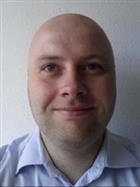
\includegraphics[scale=0.9]{Morten}}
	\hspace{1.5cm}
	\subcaptionbox*{s134000, Budtz, Christian}[6cm][c]
		{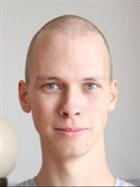
\includegraphics[scale=0.9]{Christian}}
\end{figure}
\begin{figure}[h]
	\centering
	\subcaptionbox*{s134004, Vørmadal, Rúni Egholm}[6cm][c]
		{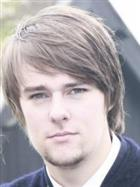
\includegraphics[scale=0.9]{Runi}}
	\hspace{1.5cm}
	\subcaptionbox*{s123064, Nielsen, Martin}[6cm][c]
		{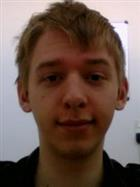
\includegraphics[scale=0.9]{Martin}}
\end{figure}
\begin{figure}[h]
	\centering
	\subcaptionbox*{s103185, Sløgedal, Magnus B.}[6cm][c]
		{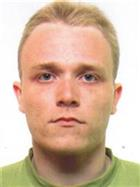
\includegraphics[scale=0.9]{Magnus}}
\end{figure}
\FloatBarrier
\end{titlepage} %%contains \thispagestyle{empty} so no numbers

\pagenumbering{arabic}		%%fixes hyperref pagenumbering error (sets it back to
\newpage					%% numbers)
\renewcommand{\figurename}{Figur}
\setcounter{figure}{0}
\tableofcontents
%\makebox[\textwidth]{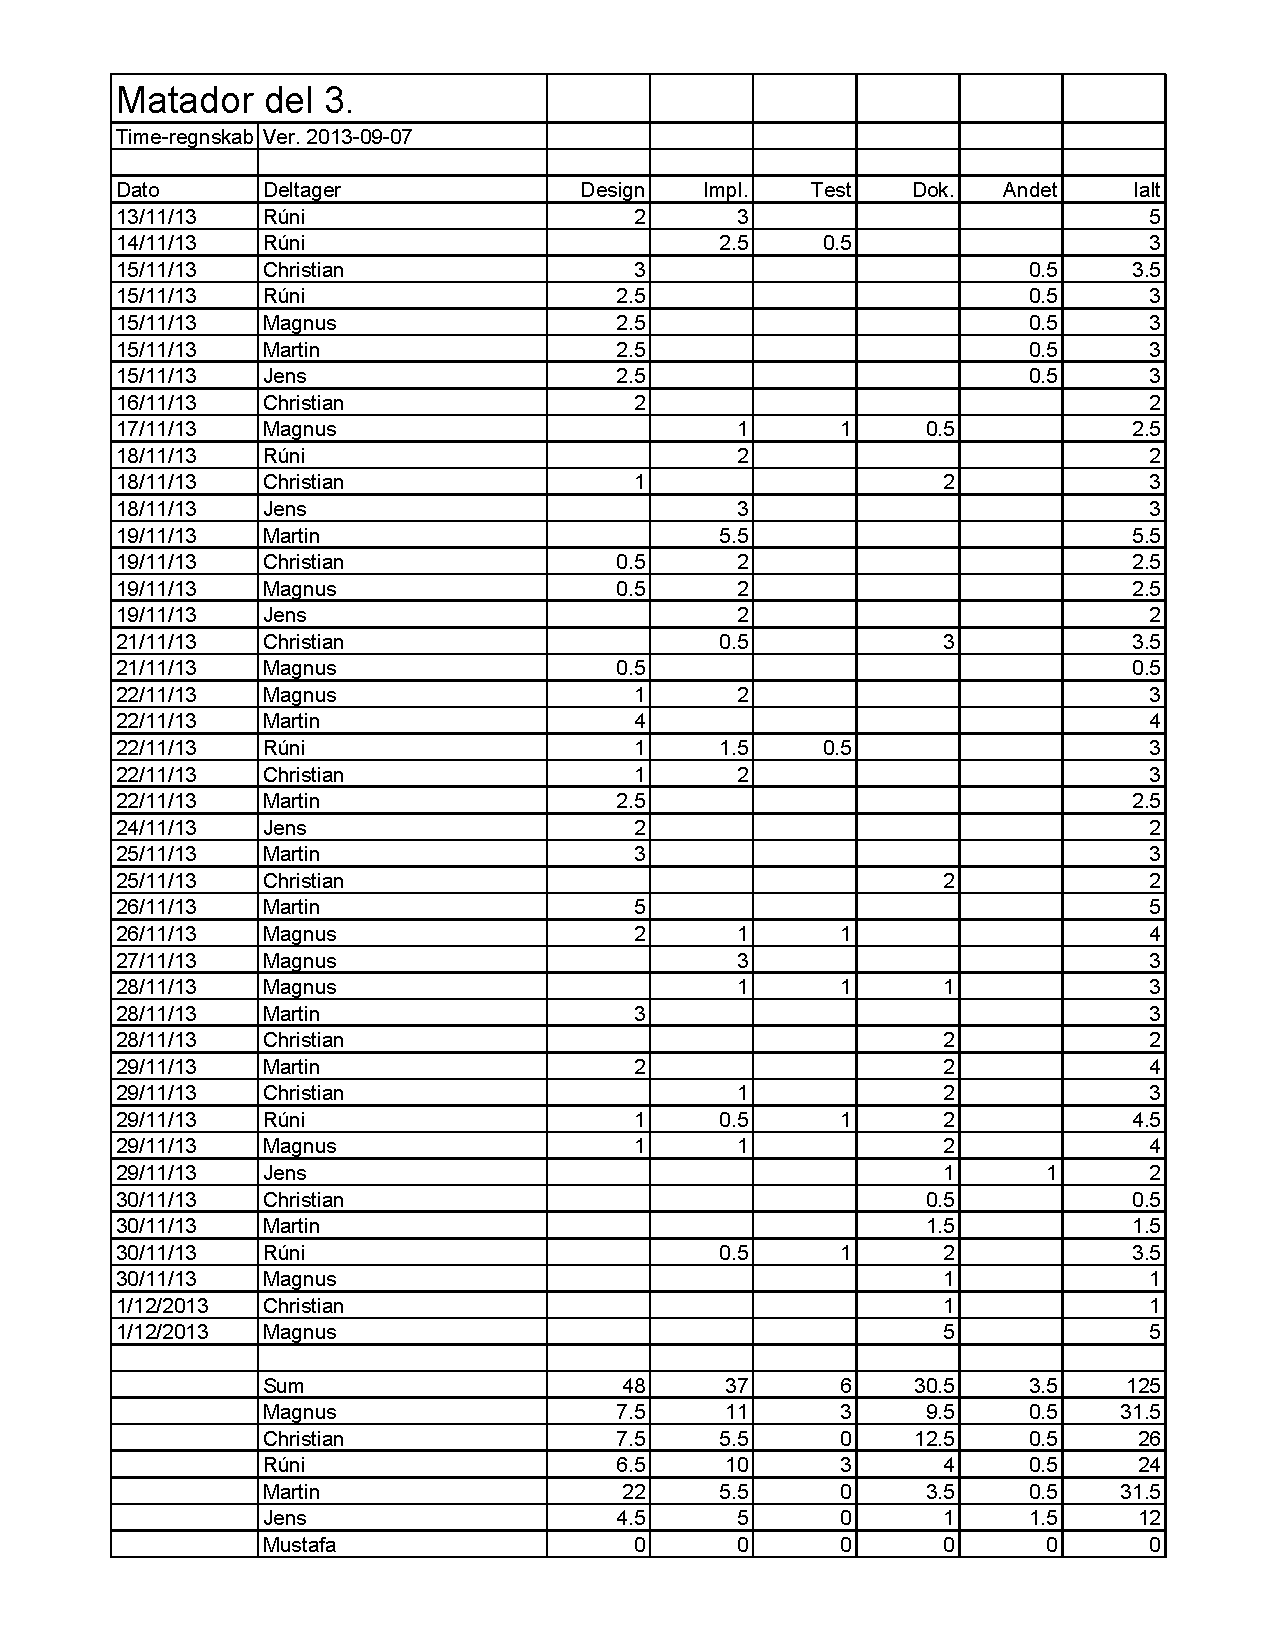
\includegraphics[width=0.7\paperwidth]{51_del3_Timeregnskab}}
\newpage
\section*{Indledning (Christian)}
\addcontentsline{toc}{section}{Indledning}
Vi har valgt at arbejde med et projekt hvor vi søger at forbedre
arbejdsgangen for røntgenrekvisitioner på Hillerød Hospital. Aktuelt fungerer
rekvisition af billeddannende undersøgelser (eks. røntgen(rtg.)billeder og MR
scanninger) via fax. Dvs. at rekvirenten (lægen), der ønsker et rtg. billede, må
sende en fax til røntgenafdelingen for at udbede sig billedet. Det skaber mange
muligheder for fejl og kan være unødigt kompliceret.
\subsection*{Kort beskrivelse af arbejdsgang (Christian, Magnus)}
\addcontentsline{toc}{subsection}{Kort beskrivelse af arbejdsgang}
I processen hvor et røntgenbillede bestilles, visiteres, bookes, udføres
og vurderes, indgår flere arbejdsgange
(se \hyperref[Rigt_billede]{figur \ref*{Rigt_billede}}).
Rekvisitionen består af en Fax (1.), der afsendes til rtg. afdelingen. Faxen
indscannes af en sekretær (2.) i et visitations/bookingsystem (- en arbejdsgang,
som vi gerne vil gøre overflødig). Herefter vurderes rekvisitionen af en
visitator (røntgenlæge), der vurderer om undersøgelsen er berettiget - visiterer
rekvisitionen (3). Herefter er rekvisitionen enten godkendt eller afvist (4.)\\
\indent Undersøgelsen bookes af en sekretær (Ikke vist). Når det planlagte
tidspunkt er nået hentes patienten fra afdelingen og patienten undersøges (5.).
Ud af undersøgelsen kommer et antal billeder, der lagres i et billedsystem (6.).
Billederne gennemses af en røntgenlæge, der skriver en  røntgenbeskrivelse (7.).
Herefter kan rekvirenten se beskrivelsen i systemet (8.).
\FloatBarrier
\begin{figure}[h]
\centering
\makebox[\textwidth]{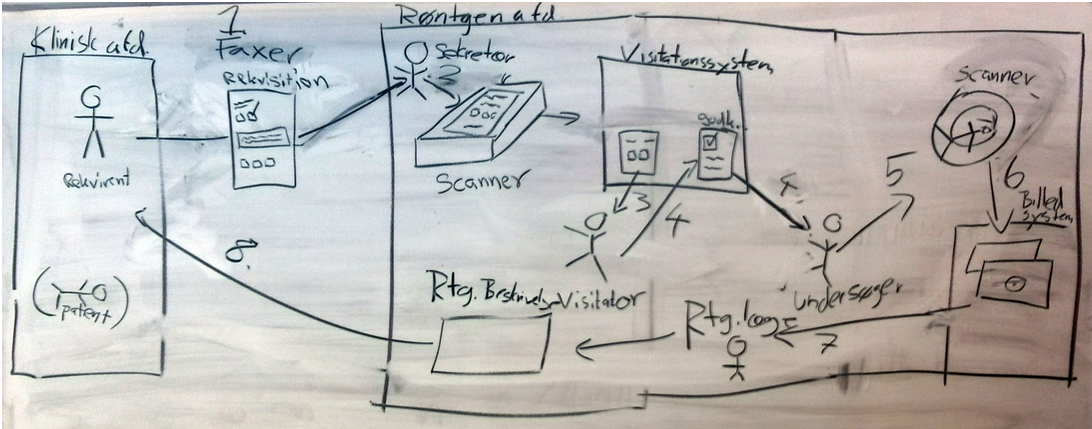
\includegraphics[width=\textwidth]{Rigt_billede}}
\caption{\emph{Rigt billede af arbejdsgangen}: Skitse udarbejdet efter
brugerbeskrivelser.\label{Rigt_billede}}
\end{figure}
\FloatBarrier
\indent Den del af processen vi interesserede os for i første omgang var selve
rekvisitions- og visitationsprocessen. Implementering af bookingsystem, og
billedbeskrivelse var for omfangsrigt til at vi kunne gå i dybden med det.
Integration med udførelsen af undersøgelsen, kræver større kendskab til det
billeddannende udstyr og deres interfaces og er urealistisk at implementere,
vores interessent-interview viste desuden at dette er en del af det nuværende
system, der fungerede godt. Røntgensvaret ligger ligeledes i det eksisterende
system, bundet til billedet, og er således heller ikke realistisk at
implementere i en rekvisitionsløsning.\\
\indent En oplagt udvidelsesmulighed var at implementere muligheden for at
rekvirenten kan se hvor langt i arbejdsgangen rekvisitionen er - om den er
modtaget, visiteret, booket m.m.
\subsection*{Proces og foranalyse (Christian, Martin)}
\addcontentsline{toc}{subsection}{Proces og foranalyse}
Vi valgte at organisere os med en projektleder og 2. leder således at
der på et hvert tidspunkt var én til at sikre at opgaver bliver udført. Desuden
uddelte vi kritiske ansvarsområder til separate medlemmer i gruppen. Vi
udformede en samarbejdskontrakt (se \hyperref[Bilag2]{bilag 2}) for at sikre at
vi havde en måde at afbøde samarbejdsproblemer.\\
\indent Vores største problemer tidligere har været at begrænse omfanget af
vores projekt og at færdiggøre delopgaver/projekt i tide - hvorfor vi har aftalt
særligt fokus på at undgå ‘feature creep’ og bedre kontrol at udviklingsflow. Vi
valgte at implementere en modificeret SCRUM backlog i forsøget på at danne os
overblik over fremdriften i projektet (se \hyperref[Bilag3]{bilag 3}). Vi satte
desuden en deadline for implementeringen- således at sidste iteration kun
drejede sig om test, bugfixing og dokumentation.
\subsubsection*{Værktøjer}
\addcontentsline{toc}{subsubsection}{Værktøjer}
Vi valgte Google Docs, Software Ideas Modeler (SIM) og Github til at håndtere
data og samarbejde, da værktøjerne før har vist sig fleksible og robuste. Vi
brugte Google Docs, da det har den fordel at vi alle kan arbejde samtidig i
dokumenter. Vi brugte SIM til at lave diagrammer, da det understøtter de fleste
af de relevante diagramtyper og vi har erfaring med værktøjet. Vi anvendte
Github, da det har vist sig driftsikkert og integreres godt med eclipse. Vi
valgte at anvende et online tool - audao\cite{audao} - til at generere
basale Data Access Objects (DAO). Det kan, fra en XML beskrivelse af
datamodellen, generere alle de nødvendige DAO og Data Transfer Objects (DTO)
klasser til databasen. CRUD operationer er således autogenererede, men mere
avancerede sql forespørgsler og triggers har vi skrevet selv. Vi valgte at
anvende HeidiSQL som interface til databasen, da vi har gode erfaringer med det.
HeidiSQL\cite{heidisql} er et brugervenligt og overskueligt opensource værktøj
til adninistraion af SQL databaser. Til bruger accept test har vi anvendt
SurveyMonkey\cite{surveymonkey} til oprettelse og hosting af spørgeskema.
\subsubsection*{Kvalitetskriterier (Magnus)}
\addcontentsline{toc}{subsubsection}{Kvalitetskriterier}
Vores kvalitetskriterier er primært at det skal være lettere og hurtigere at at
bestille en undersøgelse. Vi vil opnå begge disse ved at erstatte den nuværende
papirbaserede arbejdsgang med et digitalt system, der kan undgå repeterende
data, håndtere kontrolskemaer, og generelt lette en arbejdstung manuel
fremgangsmåde. Den bedste måde at checke om vi har opnået disse vil nok være via
et spørgeskema udleveret til brugerne, dog er det, grundet generel travlhed i
det danske sygehussystem, usikkert om vi kan få respons på dette.
\subsection*{Risikoanalyse (Rúni, Magnus)}
\addcontentsline{toc}{subsection}{Risikoanalyse}
Initielt udførte vi en risikoanalyse for at identificere de umiddelbare ricisi i
projektet, som vi skulle adressere.\\
\FloatBarrier
\begin{figure}
\begin{tabularx}{\textwidth}{| X | l | l | X | l | l |}
\hline
Risiko & Sandsynlighed & Impact & RMMM & Prioritet & RE\\ \hline
Manglende adgang til enkelte interessenter & 75\% & 5 & Afklar hurtigt hvilke
interessenter og hvad vi gør for erstatning & medium & 3,75\\
\hline

Dårlig time-estimering & 75\% & 5 & Tidsplanlægning opdateres løbende, og
eventuelt uopnåelige mål flyttes til næste iteration eller skæres fra. & medium
& 3,75\\ 
\hline \hline

Opgaven bliver for stor & 25\% & 9 & Starte med den centrale usecase og udvikle
den færdig, således at vi efter hver iteration har et færdigt produkt der kan
afleveres. & høj & 2,25\\
\hline

Begrænset adgang pga. sensitive patient data & 90\% & 2 & Begrænset betydning -
projektet kan gennemføres uden 'real life' data. & lav & 1,8\\
\hline

Manglende adgang til dokumenter & 10\% & 8 & Afklar hurtigt adgang til
dokumenter & høj & 0,8\\
\hline

Manglende erfaring / implementerings vanskeligheder & 10\% & 2 & Eventuelle
implementerings problemer løses fælles, eller kan i værste fald skæres fra. &
lav & 0,2\\
\hline
\end{tabularx}
\caption{\emph{Risiko tabel}: sorteret efter Risk Exposure.\label{risiko_tabel}}
\end{figure}
\FloatBarrier
\indent For at undgå problemet med manglende adgang til interessenter sørgede vi
allerede tidligt i vores forløb for at kontakte Hillerød hospitals
røntgenafdeling og fik en aftale i stand. Problemer med tidsplanlægningen
forsøgte vi at afbøde ved at planlægge opgaver i god tid, og bruge
tidsplanlægningsværktøjer så som en backlog og et PERT diagram. Vi prioriterede
vores mål og kunne skære de mindre væsentlige fra, da projektet kom i tidsnød.
\subsection*{Planlægning (Christian)}
\addcontentsline{toc}{subsection}{Planlægning}
Vi skabte overblik over vores projekt ved at opstille et antal veldefinerede
opgaver for den nærmeste fremtid og konstruerede et basalt PERT diagram
(se \hyperref[Bilag4]{bilag 4}) for at opklare bindinger og estimere et
tidsforbrug. Vi søgte at opdele projektet i mindre 'bidder', således at vi
arbejdede i 3 'sprints'/iterationer. Vi valgte at sætte afleveringen af vores
første prototype, udviklet som mockup i Google Forms og Excel, som første
milestone. Herefter arbejdede vi videre med kravspecifikation, analyse og design
ud fra de inputs brugerne gav os. Desuden lagde vi os fast på og startede på en
implementering i Java/jsp og MySQL. Anden milestone blev afleveringen af vores
fungerende online prototype til fornyet brugertest, hvorefter tredje iteration
blev sat af til rapportfærdiggørelse, intensivering af tests og bugfixing.

\newpage
\section{Kravspecifikation}
\subsection*{Problemformulering}
\addcontentsline{toc}{subsection}{Problemformulering}
Det eksisterende system ufleksibelt, understøtter ikke domæneregler og har meget
lav fejltolerance. Dette påvirker klinikerne og i sidste ende patienterne - da
meget tid går tabt på det eksisterende system og undersøgelser ikke bliver
udført som planlagt.\\
\indent Vi ser en mulighed for at skabe et langt sikrere og mere fleksibelt
system, hvor rekvisitioner og brugere kan spores gennem hele systemet, hvorved
risikoen for potentielt fatale fejl minimeres.\\
\indent \emph{Økonomi.} Aktuelt arbejder 3 sekretærer helt eller delvist med
håndtering af henvisninger. En stor del af arbejdsbyrden vil kunne
reduceres/elimineres og ledende sekretær skønner at der kunne frigøres minimum
én fuldtids sekretær ved en smidigere arbejdsgang. Hertil kommer tabt indtjening
som følge af aflyste/glemte undersøgelser.\\
\subsubsection*{Direkte Interessenter}
\addcontentsline{toc}{subsubsection}{Direkte Interessenter}
\begin{enumerate}
  \item Klinikere - Bestiller undersøgelser
  \item Røntgenlæger - Visiterer undersøgelser og udfører lægeundersøgelser
  \item Radiografer - Visiterer undersøgelser og udfører øvrige
  \item Sekretærer - Booker undersøgelserne
\end{enumerate}

\subsubsection*{Indirekte Interessenter}
\addcontentsline{toc}{subsubsection}{Indirekte Interessenter}
\begin{enumerate}
  \item Ledelse - Økonomiske interesser
  \item Patienter - Interesseret i at visitationen
\end{enumerate}
\subsection*{Domæne dataindsamling (Christian, Magnus)}
\addcontentsline{toc}{subsection}{Domæne dataindsamling}
For at samle mest mulig data om domænet overvejede vi de mulige måder at
indsamle data. Da der er begrænset med tid i sundhedsvæsenet, prioriterede vi
dataindsamlingsmetoder, der belastede afdelingen mindst muligt og udviklede
vores modeller/prototyper mest muligt, før vi præsenterede dem for brugerne.\\
\indent Initielt mødtes vi med en læge fra afdelingen, der gav os en
baggrundsorientering om hvordan systemet fungerer i praksis. Vi sørgede herefter
for at indsamle alle relevante dokumenter og analyserede disse (se
\hyperref[Bilag5]{bilag 5 - 9}). Vi valgte ud fra disse at lave en prototype,
før vi interviewede interessenterne for at opnå maksimalt udbytte af
interviews'ne. Da der er tale om følsomme data - patientoplysninger mm. - var
det begrænset hvad der kunne lade sig gøre mht. observationer i praksis - vi fik
lov til at se programmerne i praksis, men fik ikke lov til at tage billeder. Vi
overvejede desuden:\\
\begin{enumerate}
  \item \emph{Spørgeskemaundersøgelse} -Det var ikke praktisk ladesiggørligt at
  bruge spørgeskemaundersøgelser, da det var for tidskrævende for
  interessenterne.
  \item \emph{Workshops} - Igen for tidskrævende for vores interessenter, dog
  ville de personer vi interviewede gerne afprøve vores 2. prototype via et
  link, hvorfor vi satte en cloudløsning op til testbrug:
  (\url{http://rtgrek-area51.rhcloud.com/})
  \item \emph{Rige billeder} - Vi illustrerede arbejdsgangen med et rigt billede
  som vi verificerede med brugerne, se \hyperref[Rigt_billede]{figur \ref*{Rigt_billede}}.
  \item \emph{Forbilleder} - Vi havde ikke mulighed for at se
  alternative/sammenlignelige systemer i drift. Vi har kendskab til løsninger,
  men ikke adgang til dem.
  \item \emph{Use cases} - Vi gennemgik de udviklede use cases med
  interessenterne for at sikre os at vi havde forstået problemdomænet rigtigt.
\end{enumerate}
\subsubsection*{Prototyping (Christian, Morten)}
\addcontentsline{toc}{subsubsection}{Prototyping}
Ud fra vores baggrundsforståelse af emnet udviklede vi en prototype på en
røntgenrekvisition, som vi vil præsentere for vores interessenter, for at
afprøve om vi havde forstået domænet rigtigt (se \hyperref[Bilag10]{bilag
10} eller
\href{https://docs.google.com/forms/d/1mb5n0rR4vUuns_TXM7ai3vY1BZxPrvxd8P4NFjs5igw/viewform}{online}).
\indent Udover prototypen på rekvisitionen, har vi også lavet en prototype på
selve visitationen af rekvisitionerne. Denne blev udviklet i Excel VBA, og
skulle blot illustrere for intressenter, hvordan vi forestiller os at
brugerinterfacet kunne se ud (se \hyperref[Bilag11]{bilag 11}).
\subsubsection*{Interviews med interessenter (Christian)}
\addcontentsline{toc}{subsubsection}{Interviews med interessenter}
I første omgang lykkedes det os at få kontakt til og interviewe tre direkte
interessenter og desuden en indirekte interessent. Grundet travlhed på
afdelingen, måtte vi begrænse os til 20 minutter med hver. Vi anvendte et antal
standardiserede spørgsmål for at afdække relevante
problemstillinger\cite{designing} (se eksempel \hyperref[Bilag12]{bilag 12}). Af
pladshensyn er interview beskrivelserne i \hyperref[Bilag13]{bilag 13}.
\indent Ud fra vores interviews tilpassede vi vores krav til vores system. Det
viste sig at det største problem var tabet af rekvisitioner og en tung
arbejdsgang. Derfor valgte vi at holde fokus på at få en velfungerende
rekvisitionsarbejdsgang. Vores visitationsprototype viste sig at være meget tæt
på ønsket - med enkelte forslag til forbedringer. Rekvisitionsprototypen
afspejlede de reelle papirrekvisitioner og viste sig - i lighed med
papirudgaverne at være noget uoverskuelig. Rekvirenten så gerne at antallet af
sider der skulle udfyldes reduceredes. Vi blev desuden også opmærksom på en del
redundant data, der blev gentaget på de forskellige kontrolskemaer.
\subsection*{Aktørbeskrivelse (Rúni, Magnus)}
\addcontentsline{toc}{subsection}{Aktørbeskrivelse}
Systemet bruges af fire aktører: Klinikere (rekvirent), sekretær (booking),
røntgenlæge (visitator) og administrator. Alle fire aktører har som udgangspunkt
forskellige rettigheder, dog er systemet designet til at en bruger senere kan få
flere rettigheder hvis det bliver nødvendigt.
\begin{itemize}
  \item Administrator har lov til at oprette brugere og bestemme hvilke
  rettigheder de har, han kan ikke slette brugere, men kun gøre dem inaktive.
  Administrator skal ikke have lov til at benytte andre brugeres funktionalitet,
  hvilket gør systemet til et tillidssystem, da administrator ellers nemt kan få
  de rettigheder han vil.
  \item Rekvirenten har mulighed for at udfylde en rekvisition og de tilhørende
  kontrolskemaer. Rekvirenten kan søge på alle rekvisitioner, og hvis de
  afventer visitation eller er blevet godkendt, men ikke bookede, har han
  mulighed for at annullere rekvisitionen, uanset om han er registreret som
  rekvirent på rekvisitionen eller ej.
  \item Visitator kan se alle rekvisitoner og søge i dem, han kan visitere dem,
  skrive kommentare til sin visitation og afvise ikke fyldestgørende rekvisitioner.
  \item Sekretæren kan se alle rekvisitoner og søge i dem, han kan booke
  rekvisitioner eller sende dem til visitation hvis det er nødvendigt.
\end{itemize}
De tilladte overlap mellem brugerroller kan ses i \hyperref[Bilag14]{bilag 14}
\subsection*{Use Cases (Morten, Martin)}
\addcontentsline{toc}{subsection}{Use Cases}
I figur 3 ses en model af de involverede use cases, som vi ville arbejde med. I
forhold til den oprindelige arbejdsgang eliminerede vi en use case, hvor
sekretæren scanner rekvisition.\\
\indent Pre-conditions for alle use cases er at bruger er logget ind.
\FloatBarrier
\begin{figure}[h]
\centering
\makebox[\textwidth]{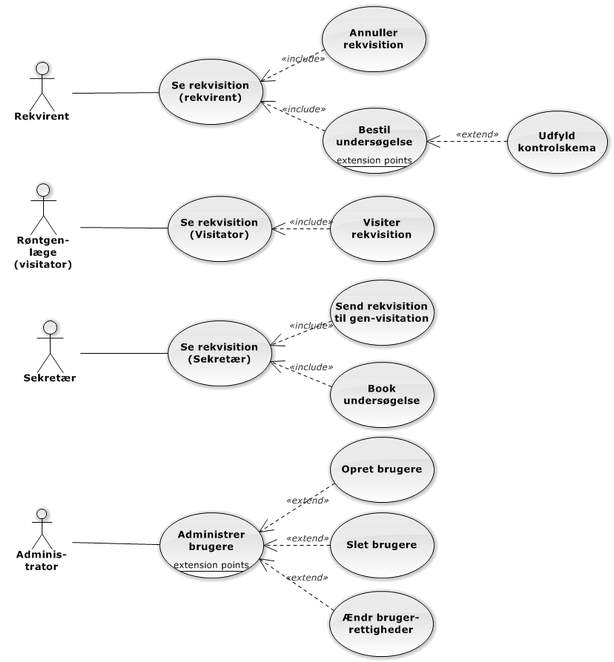
\includegraphics[width=\textwidth]{Usecase_Diagram}}
\caption{\emph{Use case diagram}: Se i øvrigt bilag 15 for tidligere version.
\label{use_case_diagram}}
\end{figure}
\FloatBarrier
\subsection*{Use case beskrivelse (fully dressed): Bestil
undersøgelse\cite{cockburn} (Martin, Morten)}
\addcontentsline{toc}{subsection}{Use case beskrivelse}
\textbf{Primær aktør:} Læge(Rekvirent)\\
\textbf{Mål:} Få en tid til en undersøgelse af en patient.\\
\textbf{Scope:} Rekvisitionssystem til Hillerød hospital.\\
\textbf{Stakeholders and interests:}
\begin{itemize}
  \item Rekvirenter: Vil have en nem, hurtig og sikker måde at sende
  rekvisitioner.
  \item Patienter: Vil komme hurtigt til undersøgelse, og være sikre på at deres
  rekvisition ikke går tabt i systemet samt minimum risiko for fejl i rekvisitionen.
  \item Visitatorer(radiolog): Vil have at data er indtastet korrekt, og er nemt
  at søge i.
  \item Radiografer: Vil have data korrekt indtastet, så de kan lave den rigtige
  undersøgelse.
  \item Sekretærer: Vil gerne have at data er indtastet korrekt i rekvisitionen.
  \item Administratorer: Vil have et sikkert og velfungerende system.
  \item Hillerød hospital: Vil skære unødvendige arbejdstimer for at spare
  penge, og have et sikkert system, da mange rekvisitioner i øjeblikket går tabt
  pga. dårligt system.
  \item Skatteyderen: Vil have deres skattepenge brugt optimalt.
\end{itemize}
\textbf{Precondition:} Alle aktører er logget ind.\\
\textbf{Minimum garanti:} Rekvisition bliver afsendt.\\
\textbf{Success garanti:} Rekvisitionsoplysninger er korrekt indtastet og
afsendt, visitatoren har godkendt rekvisitionen, sekretæren har booket en tid,
data er gemt i systemet.\\
\textbf{Main success scenario:}
\begin{enumerate}
  \item Rekvirent logger ind
  \item Opretter en rekvisition
  \item Indtaster oplysninger i rekvisitionen, og vælger den rigtige modalitet
  \item Udfylder evt. kontrolskema og trykker submit
  \item En visitator logger ind
  \item Vælger den pågældende rekvisition
  \item Godkender undersøgelsen
  \item Sekretæren logger ind
  \item Vælger den pågældende godkendte rekvisition
  \item Booker en undersøgelse til patienten.
\end{enumerate}
\textbf{Extensions:}
\begin{description}
\item[*a)]Hvis systemet går ned, genstartes webserveren af IT-afdelingen.
\item[2-4a)]Hvis brugeren er i gang med at indtaste en rekvisition, og vil
fortryde oprettelsen, kan dette ske ved enten at lukke rekvisitionen på det
store X eller trykke på ESC på tastaturet.
\item[6-7a)]Hvis to visitatorer åbner samme rekvisition, kan den kun godkendes
eller afvises én gang.
\begin{enumerate}
  \item Den visitator der godkender/afviser sidst, får at vide at rekvisitionen
  allerede er behandlet.
  \item Rekvisitionens status ændres ikke.
\end{enumerate}
\item[9-10a)] Hvis to sekretærer forsøger at behandle den samme rekvisition
(booke/send til visitation), kan kun den ene behandle den.
\begin{enumerate}
  \item Den sekretær der forsøger at behandle rekvisitionen sidst, får at vide
  at den allerede er behandlet.
  \item Rekvisitionens status ændres ikke.
\end{enumerate}
\end{description}
Ikke alle extensions er listet, da det ville tage for meget plads i rapporten.
\textbf{Trigger:} En læge åbner rekvisitionsiden for at bestille en
billeddannende undersøgelse.\\
\indent For yderligere use case beskrivelser, se \hyperref[Bilag16]{bilag 16}.
\subsection*{Domæneregler (Morten)}
\addcontentsline{toc}{subsection}{Domæneregler}
Vores system skal kunne understøtte særlige domæneregler.
\subsubsection*{Domæneregel “Over 18”}
\addcontentsline{toc}{subsubsection}{Domæneregel “Over 18”}
Når patienten er over 18 og der er valgt “Røntgen” under modalitet, skal
rekvisition ikke visiteres. Det vil sige at den bookes direkte uden forudgående visitation.
\subsubsection*{Domæneregel “Adskillelse af rekvirent og visitator”}
\addcontentsline{toc}{subsubsection}{Domæneregel “Adskillelse af rekvirent og visitator”}
I den nuværende setting er det ikke tilladt visitatorer at rekvirere en
undersøgelse og omvendt heller ikke tilladt en rekvirent at kunne visitere
rekvisitioner. Denne regel betyder at rekvirenten ikke kan visitere de
rekvisitioner, vedkommende selv har oprettet. Dette er for at sikre mod
vennetjenester, samt at sikre at det kun er klinikere (med behandlingsansvar for
patienten) der bestiller røntgenundersøgelser. Paraklinikerne bør ikke på eget
initiativ iværksætte andre undersøgelser. Se evt. \hyperref[Bilag14]{bilag 14}.
\subsection*{Supplerende krav - FURPS+ (Christian)}
\addcontentsline{toc}{subsection}{Supplerende krav - FURPS+}
Udfra vores indsamlede data kunne vi sammenfatte et antal krav, der ikke er
indfattet i vores use cases.
\subsubsection*{Funktionelle krav}
\addcontentsline{toc}{subsubsection}{Funktionelle krav}
\begin{enumerate}
  \item Der skal være sporbarhed, således at en røntgenrekvisition altid kan
  genfindes og rekvirent, visitator og booker skal kunne genfindes -
  Rekvisitioner må ikke slettes.
  \item Alle brugere skal logge ind med kodeord, da der er tale om følsomme
  data.
\end{enumerate}

\subsubsection*{Non-funktionelle krav}
\addcontentsline{toc}{subsubsection}{Non-funktionelle krav}
\textbf{Usability}
\begin{enumerate}
  \item Arbejdsgangen med røntgenrekvisitionen skal overordnet være nemmere end
  nuværende arbejdsgang, således at der er incitament for at bruge det
  nyudviklede system fremfor det gamle. Dette kan måles via et spørgeskema -
  hvilket nok vil give det mest retvisende billede, da det er den oplevede
  nemhed der er betydende. Et tilbagevendende kritikpunkt var de mange klik i
  hver arbejdsgang og den lange ventetid imellem klik. Antallet af klik i
  arbejdsgangen kan tælles direkte ved at gennemføre en arbejdsgang med enten
  det nye eller gamle system. Ventetiden kan tilsvarende måles eks. ved at
  gennemføre et antal rekvisitioner på repræsentative tidspunkter med hhv. det
  nye og det gamle system.
  \item Selve udfyldningen af rekvisitionen fungerer aktuelt godt, da
  papirrekvisitionen er valideret og optimeret over flere år. Det er dog
  kompliceret at der skal medsendes kontrolskemaer til nogle undersøgelser - de
  går ofte tabt. I vores system, kan en forbedring være at kontrolskemaer bliver
  vist automatisk afhængigt af hvilken undersøgelse der bliver valgt.
  \item Nogle felter på rekvisitionen skal ikke udfyldes afhængigt af andre
  felter - eksempelvis, skal ambulant transport ikke udfyldes, hvis patienten er
  indlagt. I en computerbaseret løsning vil de obsolete felter kunne udelades
  dynamisk, hvilket vil forbedre brugeroplevelsen.
\end{enumerate}
\textbf{Reliability}
\begin{enumerate}
  \item Systemet er et kritisk system, forstået på den måde at længerevarende
  nedbrud kan resultere i at undersøgelser bliver forsinket. Kortere nedbrud vil
  ikke forstyrre driften, da akutte undersøgelser stadig kan gennemføres, og det
  eksisterende system kan tage over. Afdelingen har ikke selv specificeret hvad
  en acceptabel 'nedetid' er, men klarer sig aktuelt med et dagligt lukkevindue
  på 10 minutter, hvor det nuværende system genstartes for at sikre stabilitet
  af systemet, hvorfor en tilsvarende daglig sammenhængende 'nedetid' også vil
  være acceptabelt - omend vi meget gerne vil forbedre dette - vi satser på en
  løsning med mindre end ét nedbrud ugentligt, hvor systemet kan være oppe igen
  indenfor 5 minutter.
  \item I det nuværende system tabes mange data (rekvisitioner) dagligt, hvilket
  er uacceptabelt i et system, der håndterer patienters behandling og
  diagnostisk - særligt når man som bruger ikke har mulighed for at se om
  rekvisitionen fortsat eksisterer/er under behandling. Vi vil gerne garantere
  at patient data ikke tabes og at man som minimum kan følge sin rekvisition og
  se dens 'vej i gennem systemet'.
\end{enumerate}
\textbf{Performance}
\begin{enumerate}
  \item For at kunne opnå en bedre brugeroplevelse med hurtigere arbejdsgange,
  skal vores løsning kunne returnere data hurtigt. Da den nuværende
  faxarbejdsgang tager flere minutter, er det i hvertfald acceptabelt med
  svartider fra serveren på sammenlagt 15 sekunder for en hel use case 'bestil
  røntgen'.
  \item Med stigende antal rekvisitioner kan forventes et større pres på
  databasen. Hillerød hospital håndterer årligt 217.000 røntgen
  undersøgelser\cite{nordhospital}, med betydelig døgnvariation. Vi estimerer at
  man skal kunne bestille op til 2000 undersøgelser dagligt uden nedetid og mærkbar forsinkelse - vi definerer
  mærkbar forsinkelse som en forlængelse af svartiderne på mere end 100\%.
  \item Med stigende antal brugere skal systemet tilsvarende ikke køre
  væsentligt langsommere. Hillerød Hospital har 17 kliniske afdelinger der
  sender røntgenrekvisitioner, hertil kommer i størrelsesordenen 100
  praktiserende læger, der sender  i størrelsesordenen 500 rekvisitioner
  dagligt. I værste fald kan vi opleve op mod 100 samtidige brugere - hvilket
  systemet skal kunne håndtere uden at gå ned eller have væsentlige
  performancetab - Igen defineret som forlængelse af svartider på over 100\%.
\end{enumerate}
\textbf{Supportability}
\begin{enumerate}
  \item Business logikken ændres løbende - eks. bliver ikke alle
  røntgenrekvisitioner visiteret. Almindelige røntgenbilleder af voksne
  visiteres ikke, men bookes med det samme. Tilsvarende regler skal kunne
  implementeres uden at omskrive programmet.
  \item Systemet kan potentielt udvides til at omfatte andre undersøgelser og
  afdelinger, hvorfor det er væsentligt med en databasestruktur, der tillader
  udvidelser uden total omskrivning af kodebasen.
\end{enumerate}
\subsubsection*{Plus}
\addcontentsline{toc}{subsubsection}{Plus}
\textbf{Designkrav}
Den grafiske udformning af rekvisitionen skal ligne den nuværende, således at
rekvirenterne ikke føler at der er for store ændringer i processen.
\textbf{Implementeringskrav}
Systemet skal kunne anvendes på mange forskelligartede computere og kunne
anvendes uden installation.
\textbf{Lovmæssige Krav}
Vi arbejder med personfølsomme data, hvorfor det er et krav at
personoplysninger\cite{retsinfo} ikke opbevares udenfor EU (ellers skal der
indhentes særskilt tilladelse).
Ligeledes er der krav om at data overføres krypteret\cite{datatilsyn}.
\FloatBarrier
\begin{figure}
\subsubsection*{Krav-interessent tabel (Magnus)}
\addcontentsline{toc}{subsubsection}{Krav-interessent tabel}
\centering
\begin{tabular}{|c|c|c|c|c|c|c|c|}
\rot{ } & \rot{Se rekvisition}& \rot{Bestil røntgen} & \rot{Visiter rekvisition}
& \rot{Book undersøgelse} & \rot{Administrer brugere} & \rot{Sporbarhed} &
\rot{Driftssikkerhed}\\
\hline
Klinikere    & X & X &   &   & X & X & X \\
\hline
Røntgenlæger & X &   & X &   & X &   & X \\
\hline
Radiografer  & X &   & X &   & X &   & X \\
\hline
Sekretærer   & X &   &   & X & X & X & X \\
\hline
Ledelse      &   &   &   &   & X & X & X \\
\hline
Patienter    &   & X &   &   &   & X &   \\
\hline
\end{tabular}
\caption{\emph{Krav-interessent tabel}: Ikke alle krav er medtaget af hensyn til
overblikket..\label{krav_interresent_tabel}}
\end{figure}
\FloatBarrier
I Krav-interessent tabllen ses et overlap mellem Radiografer og Røntgenlæger,
hvorfor disse også slås sammen som 'Visitatorer'.
\subsubsection*{Kravprioritering - MoSCoW (Christian)}
\addcontentsline{toc}{subsubsection}{Kravprioritering - MoSCoW}
\indent\emph{Must have.}Af vores use cases er 'Bestil røntgen', 'Visiter
rekvisition' og 'Book undersøgelse' essentielle for brugen af systemet.\\
\emph{Should have.} Muligheden for at følge rekvisitionen er væsentlig og
dermed også 'Se rekvisition'. Systemet bør overholde lovkrav. Data bør ikke
slettes i databasen, af hensyn til sporbarheden. Systemet er kritisk og bør have
en høj oppetid.\\
\emph{Could have.} 'Send rekvisition til gen-visitation' og 'Annuller
rekvisition' er vigtigt i det normale arbejdsflow, men kan undværes.
Kontrolskemaer går ofte tabt, og en implementering 'Udfyld kontrolskema' vil
betyde meget for patientsikkerheden. 'Administrer brugere' vil være godt at
implementere som en bruger funktionalitet, men kan håndteres direkte i
databasen, da der vil være begrænset udskiftning i brugerne. Domæneregler vil
lette arbejdsgangen, men er nonessentielle. Øvrige non-funktionelle krav er i
denne kategori.\\
\emph{Want to have.} Ledelsen så gerne muligheden for at trække
statistikker over de forskellige visitatorers og rekvirenters 'forbrug' af
rekvisitioner. Dette er ikke betydende for funktionaliteten.


\newpage
\section{Analyse}
Kundens vision er at få leveret et terningspil, der kan spilles af 2-6 spillere.
Spillerne rykker rundt på et ringformet spillebræt med 21 felter. Hver spiller
starter med 30.000. Spillet slutter når kun en spiller ikke er bankerot.\\
\FloatBarrier
\begin{figure}[h]
\section*{Domænemodel}
\addcontentsline{toc}{subsection}{Domænemodel}
\centering
\makebox[\textwidth]{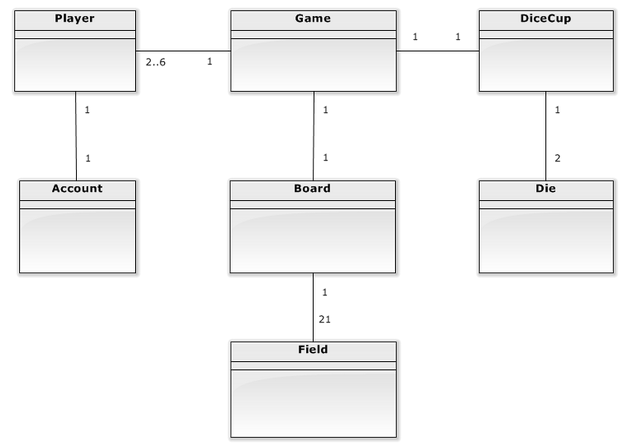
\includegraphics[width=\textwidth]{DOM_51_del3}}
\caption{\emph{Domæne model}: Viser hvordan spillet hænger sammen ude i den
virkelige verden. Det man ikke kan se her, er at Field, indeholder forskellige slags
felter.}
\end{figure}
\FloatBarrier
\section*{Use Cases}
\addcontentsline{toc}{subsection}{Use Cases}
Vi har valgt at betragte spillet som bestående af en overordnet spil ‘use case’,
hvor spillerne efter tur slår med terninger og rykker rundt på felterne. Vi
betragter hvert ophold på et felt som en separat sub use case, der igen udvides
i flere trin (se Use case diagram). Nogle af felterne kan ejes og modelleres
derfor i en separat use case - der igen er delt op i flere typer af felter - alt
efter hvordan lejen af feltet afgøres.\\
\indent Af kunden er det specificeret at netop ‘Land on Fleet’ skal være særligt
grundigt dokumenteret - ‘fully dressed’. Vi har valgt at beskrive en sub use
case, ‘Land on Field’, der er højere i hierarkiet, som ‘fully dressed’, idet der
er mange generelle elementer, der går igen i de forskellige use cases. ‘Land on
Fleet’ er således beskrevet som en extension af den mere generelle ‘Land on
Ownable Field’, der igen er et specialtilfælde af ‘Land on Field’.\\
\FloatBarrier
\begin{figure}[h]
\section*{Use Case Diagram}
\addcontentsline{toc}{subsection}{Use Case Diagram}
\centering
\makebox[\textwidth]{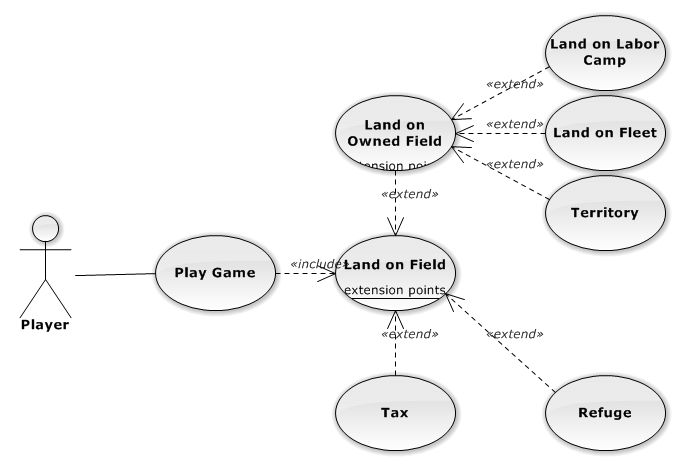
\includegraphics[width=\textwidth]{Usecasediagram1}}
\caption{\emph{Use Case Diagram}: Vi har valgt at beskrive ‘Land on Field’ som
en include i Play Game - selvom der ikke er flere use cases der include’r ‘Land on
Field’. Dette er gjort for at synliggøre relationen mellem sub use cases.}
\end{figure}
\FloatBarrier
\section*{Main Use Case ‘Spil Terningspil’}
\addcontentsline{toc}{subsection}{Main Use Case ‘Spil Terningspil’}
\begin{enumerate}
  \item Spillerne starter spillet og vælger hvor mange spillere de vil være.
  \item De indtaster spillernavne.
  \item Spillerne starter med 30000 points hver. Spillebrættet har 21 felter,
  der ligger i en ring. Nogle af felterne kan ejes af spillerne.
  \item Spillerne slår efter tur med 2 terninger og rykker summens øjne frem på
  spillebrættet. Alt efter hvilket felt man lander på mister eller får man penge
  og en ejer modtager evt. pengene. Se sub use case ‘Land on Field’
  \item Spillet slutter når alle undtagen én spiller er fallit og den
  tilbageværende spiller vinder.
\end{enumerate}
\textbf{Extension:}\\
1a. Spillerne kan vælge sprog\footnote{Er ikke specificeret i oplægget, men vi
har valgt at implementere det, som en ekstra udfordring.}.\\
\\
\textbf{\large Sub Use Case ‘Land on Field’ (fully dressed)}\\
Included in Main Use Case (4.)\\
\textbf{Scope:} Terningspil.\\
\textbf{Level:} Subfunction.\\
\textbf{Primary Actor:} Aktive spiller (spilleren der har tur).\\
\textbf{Stakeholders and Interests:} Alle spillere:
\begin{itemize}
  \item Er interesserede i at spillerne får opdateret deres pengebeholdning i
  overensstemmelse med reglerne for felttypen.
  \item Er interesserede i at finde ud af om den aktive spiller går fallit.
  \item Forventer entydig kommunikation af resultatet af at lande på feltet.
\end{itemize}
\textbf{Preconditions:} Spillet er startet og der er en aktiv spiller (der har
turen), der lander på et felt.\\
\textbf{Postconditions:} De involverede spillers pengebeholdning bliver
opdateret. Spillerens tur afsluttes.\\
\textbf{Main Success Scenario:}
\begin{enumerate}
  \item Spilleren lander på feltet.
  \item Spillerens penge beholdning opdateres.
  \item Spillerens tur afsluttes.
\end{enumerate} 
\textbf{Extensions:}\\
2a. Feltet kan ejes - Sub Use Case Land on Ownable Field.\\
2b. Feltet er af typen ‘Tax’ - Sub Use Case Land on Tax.\\
2c. Feltet er af typen ‘Refuge’ - Sub Use Case Land on Refuge\\
2d. Spilleren går fallit
\begin{enumerate}
  \item Spillerens penge sættes til 0.
  \item Spilleren får ikke flere ture.
\end{enumerate}
\textbf{Special Requirements, Technology and Data variations list.}\\
Der er i den givne opgave ikke stillet krav inden for ovenstående.\\
\textbf{Frequency of occurrence.}\\
Hver runde i spillet.\\
\textbf{Open Issues.}\\
Beskrevet under afklaring og antagelser.\\
\\
\textbf{\large Sub Use Case Land on Ownable Field}\\
Extends \emph{Land on Field.}\\
Feltet kan ejes.
\begin{enumerate}
  \item Feltet har ingen ejer.
  \begin{enumerate}
    \item Spilleren tilbydes at købe feltet, har tilstrækkeligt med penge og
    køber feltet.
    \begin{enumerate}
      \item Spilleren bliver ejer af feltet.
      \item Prisen for feltet fratrækkes spillerens saldo.
    \end{enumerate}
    \item Spilleren tilbydes at købe feltet, har tilstrækkeligt med penge, men
    køber ikke feltet.
    \item Spilleren har ikke tilstrækkeligt med penge til at købe feltet.
  \end{enumerate}  
  \item Feltet er allerede ejet af spilleren.
  \item Feltet er ejet af en anden spiller.
  \begin{enumerate}
    \item Spilleren betaler leje til ejeren.
  \end{enumerate}
\end{enumerate}
\textbf{Extensions:}\\
3.1a. Feltet er et ‘Territory’ - Sub Use Case Land on Territory.\\
3.1b. Feltet er et ‘Labor Camp’ - Sub Use Case Land on Labor Camp.\\
3.1c. Feltet er et ‘Fleet’ - Sub Use Case Land on Fleet.\\
3.1d. Spilleren har ikke tilstrækkeligt med penge til at betale ejeren.
\begin{enumerate}
  \item Ejeren får spillerens resterende penge.
  \item Spilleren går fallit.
\end{enumerate}
\\
\textbf{\large Sub Use Case Land on Territory}\\
Extends \emph{Land on Ownable Field.}\\
1. Spilleren der lander på ‘Territory’ betaler ejeren et foruddefineret
beløb.\\
\\
\textbf{\large Sub Use Case Land on Labor Camp}\\
Extends \emph{Land on Ownable Field.}\\
1. Spilleren der lander på ‘Labor Camp’ betaler ejeren 100 gange øjnene på det
slag, der har bragt ham til feltet.\\
\\
\textbf{\large Sub Use Case Land on Fleet}\\
Extends \emph{Land on Ownable Field.}\\
1. Spilleren der lander på ‘Fleet’ betaler ejeren $2^n \cdot 250 $, hvor n er
antallet af fleets, som ejeren ejer.\\
\\
\textbf{\large Sub Use Case Land on Tax}\\
Extends \emph{Land on Field.}\\
1. Spilleren mister et foruddefineret beløb.\\
\textbf{Extension:}
1a. På nogle ‘Tax’ felter kan spilleren i stedet vælge at betale en procentdel
af sin samlede formue\\
\\
\textbf{\large Sub Use Case Land on Refuge}\\
Extends \emph{Land on Field.}\\
Spilleren modtager et foruddefineret beløb.\\
\section*{Non funktionelle krav}
\addcontentsline{toc}{subsection}{Non funktionelle krav}
I den givne opgave er der det er et krav at der er udarbejdet
Kravspecificering:
\begin{enumerate}
  \item Et use-case diagram og use-case beskrivelser. Som minimum skal ”Land on
  fleet” være fully dressed.
  \item Domæne-model og BCE-diagram
\end{enumerate}
Kodemæssigt forlanges:
\begin{enumerate}
  \item Lav passende konstruktører.
  \item Lav passende get og set metoder.
  \item Lav passende toString metoder.
  \item Lav en klasse GameBoard der kan indeholde alle felterne i et array.
  \item Tilføj en toString metode der udskriver alle felterne i arrayet.
  \item Lav en Junit test til hver af felttypernes ”landOnField”-metode.
  \item Lav det spil kunden har bedt om med de klasser I nu har.
  \item Benyt den udleverede GUI.
\end{enumerate}
Designmæssigt forlanges:
\begin{enumerate}
  \item DSD’er (Design Sekvens Diagrammer). Som minimum ”Land on fleet”.
  \item Forklaring af arv, keywordet abstract, og konceptet i at implementere
  landOnField metoder i både super og subclasses (override).
  \item Dokumentation for test med screenshots.
  \item Dokumentation for overholdt GRASP.
\end{enumerate}
\section*{Afklaring og antagelser}
\addcontentsline{toc}{subsection}{Afklaring og antagelser}
\begin{enumerate}
  \item Vi adspurgte kunden om felterne skulle ligge i nummereret rækkefølge på
  brættet. Kunden svarede at det var valgfrit, men så gerne at de lå tilfældigt.
  \item Vi antager at alle spillere starter på første felt
  \item Vi antager at alle felter bevarer deres værdi når de er købt - således
  at det koster 10\% af ens saldo + 10\% af indkøbsprisen for de Tax felter hvor
  det er muligt at betale 10\% af sin formue.
\end{enumerate}
\section*{Ikke honorerede krav}
\addcontentsline{toc}{subsection}{Ikke honorerede krav}
Vi har forsøgt at honorere alle krav.\\

\newpage
\section{Design}
Ud fra ovenstående use case analyser er vi fortsat med at designe en løsning på
opgaven. I lighed med den foregående opgave har vi besluttet os for en løsning
med en decorator, der sørger for at gøre det let at oversætte spillet til et
andet sprog. I vores tilfælde har vi en lidt speciel GUI, der - imodsætning til
en ‘normal’ GUI - afventer en forespørgsel fra vores Gamecontroller/Decorator.
Dette afspejles i vores BCE diagram. I vores BCE diagram er lagt op til en
central controller, hvilket vi dog har valgt at ‘bøje’ lidt i
klassediagrammet.\\
\FloatBarrier
\begin{figure}[h]
\section*{BCE Diagram}
\addcontentsline{toc}{subsection}{BCE Diagram}
\centering
\noindent 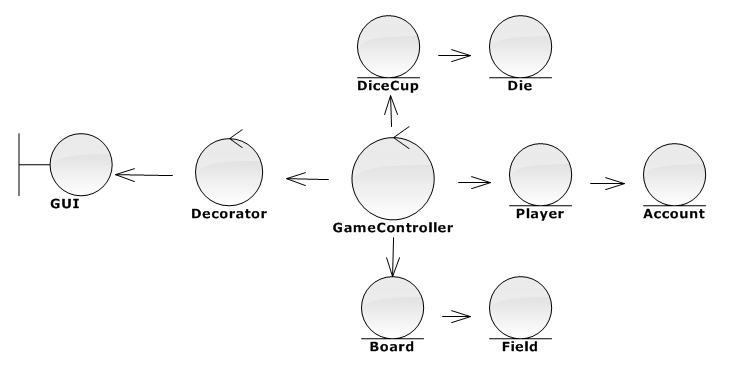
\includegraphics[width=\linewidth]{Robustnessdiagram1}
\caption{\emph{BCE diagram}: Bemærk den lidt usædvanlige
relation mellem GameController Decorator og GUI. GUI afventer en forespørgsel
fra Gamecontroller/Decorator, hvorfor pilen vender modsat vanlig interaktion med
en GUI.}
\end{figure}
\FloatBarrier
\begin{figure}[h]
\section*{Design Klasse diagram}
\addcontentsline{toc}{subsection}{Design Klasse Diagram}
\centering
\noindent 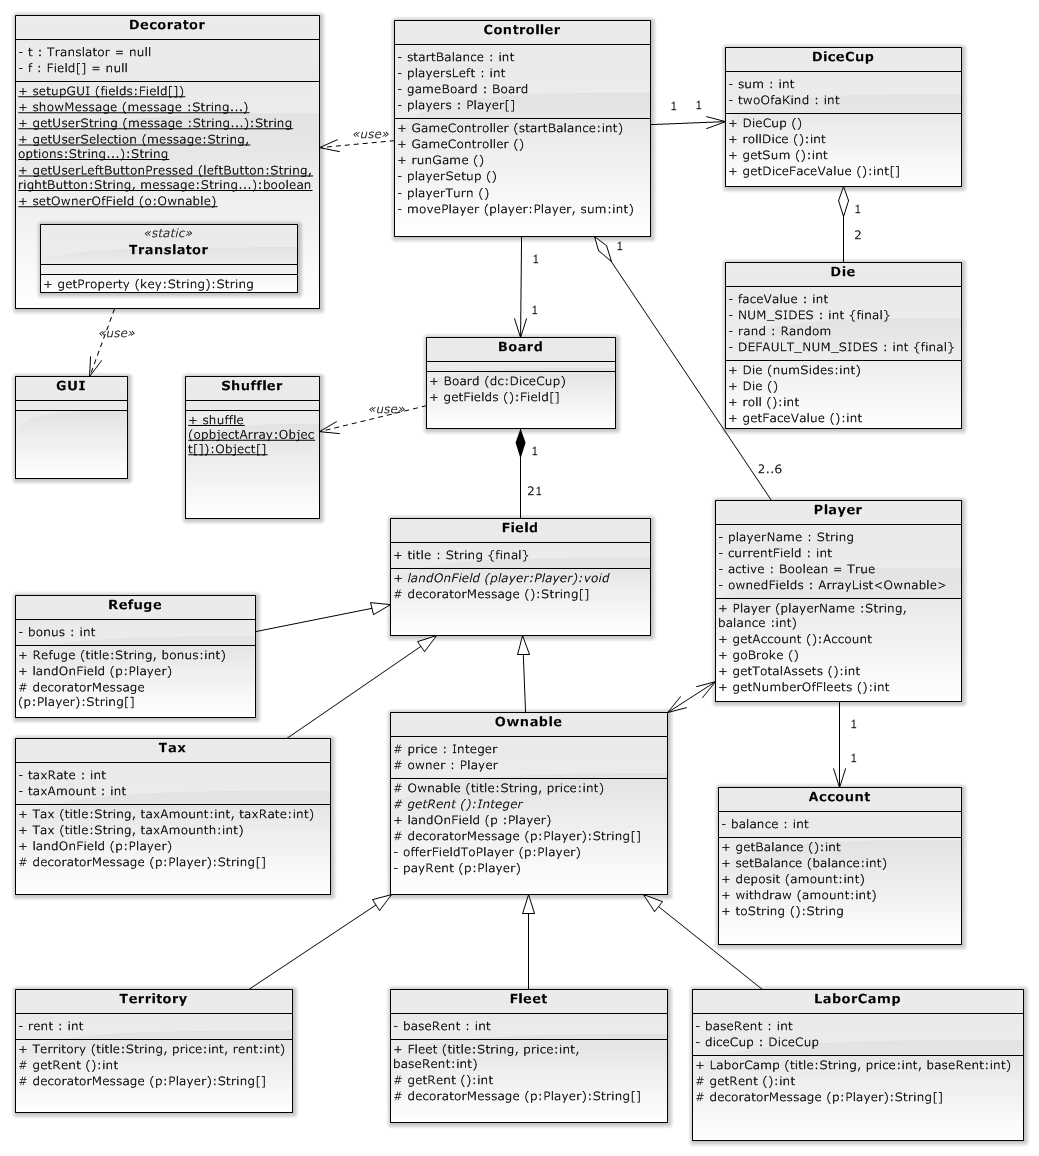
\includegraphics[width=\linewidth]{Classdiagram1}
\caption{\emph{Design klasse diagram}: Flere ‘use’ relationer er udeladt for
overskuelighedens skyld. Således er der en ‘use’ relation fra Refuge, Tax,
Territory, Fleet, LaborCamp og Player til Decorator, der er en statisk klasse og
dermed kan tilgås globalt. Desuden er udeladt en association fra LaborCamp til
DiceCup, der bruges til at tilgå terningslaget.\\
I design klassediagrammet har vi udviklet BCE modellen yderligere, så
den rent faktisk afspejler koden. Der er dukket to nye hjælperklasser op - Shuffler og
Translator, der er henholdsvis en statisk hjælperklasse, der kan blande objekter
i et array og en indre klasse, der oversætter Strings via en properties fil,
der er sprogspecifik.}
\end{figure}
\FloatBarrier
\section*{Arv, Polymorfi og Abstract}
\addcontentsline{toc}{subsection}{Arv, Polymorfi og Abstract}
Klassen Field er nu videreudviklet til at have et arvehieraki, der reflekterer
at Fields er forskellige, men har ensartede attributter og metoder - altså
udviser polymorfi. Polymorfi er: \emph{“Muligheden for at bruge den samme kode på
flere forskellige objekter, og for at den kode kan opføre sig forskelligt alt
efter hvilket objekt der er tale om.”}\cite{buildingJava} I vores kode bruger vi
polymorfi til at differentiere mellem forskellige felters landOnField metode, og
vi bruger det i decoratorMessage til at bestemme hvilket text output, der skal
sendes til vores Decorator og videre til GUI.\\
\indent Alle felterne har attributten ‘title’ tilfælles, hvorfor den ligger i
øverste klasse ‘Field’ i arvehierarkiet. Desuden implementerer Field metoden
decoratorMessage(), og en abstrakt metode - landOnField(). Det at en metode er
abstrakt, betyder at den ikke bliver  implementeret i den klasse hvor den er
erklæret abstrakt - det vil sige den ikke  har en metode-body. Fordelen ved at
erklære en abstrakt metode i superklassen er  at man tvinger sub klasser til at
implementere klassen, og man derfor kan være  sikker på at alle subklasser har
metoden. Når en metode bliver erklæret abstrakt  skal klassen også erklæres
abstract. For en klasse betyder dette at den ikke  længere kan instantieres, så
hvis man skal bruge den bliver man nødt til at  nedarve den til en sub-klasse.\\
\indent Ownable er super klasse for de felter  der kan købes - og en sub klasse
af Field. Det er meningsfyldt, da de alle skal  kunne købes - altså har en pris,
‘price’ og en ejer ‘owner’ og skal implementere  metoder til at beregne leje -
getRent().\\
\indent Med de to super klasser Field og  Ownable har vi opnået at kunne
genbruge så meget kode som muligt og undgår  dermed at skulle rette flere steder
i koden når metoderne skal opdateres.\\
\FloatBarrier
\section*{Sekvensdiagrammer}
\addcontentsline{toc}{subsection}{Sekvensdiagrammer}
Ud fra uses cases og klasse diagram har vi forsøgt at analysere flowet i spillet
og modelleret det i de følgende sekvensdiagrammer.
\begin{figure}[h]
\centering
\noindent 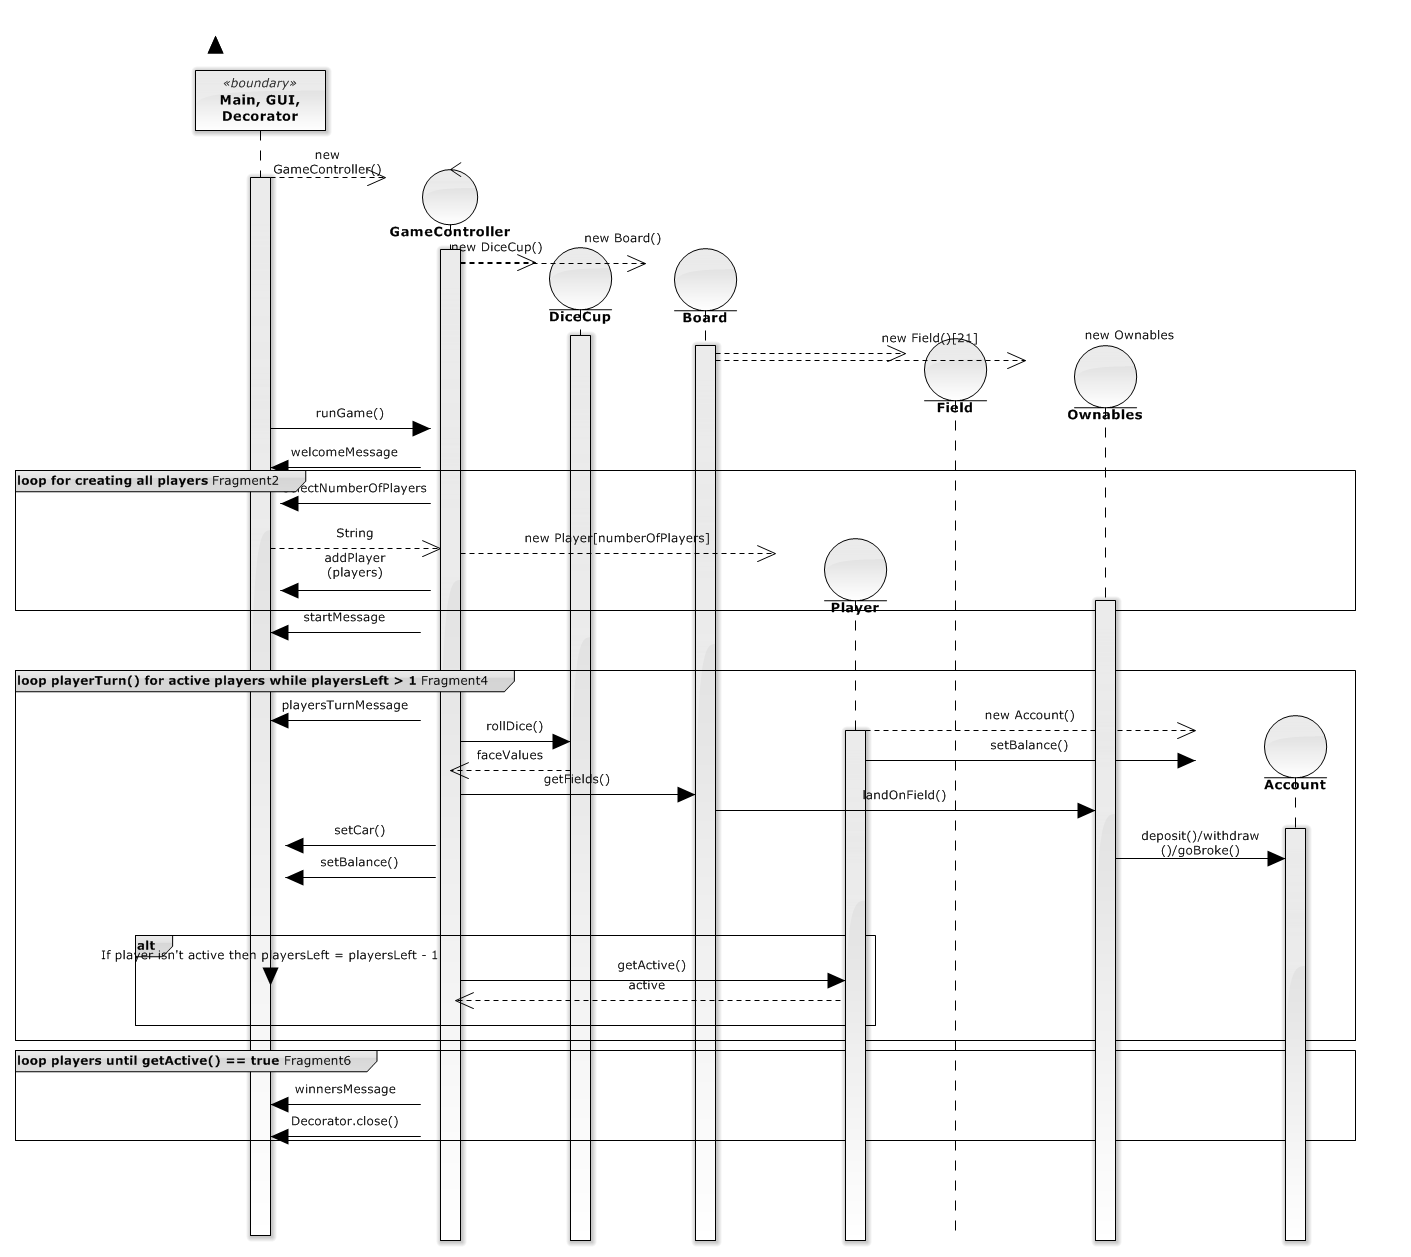
\includegraphics[width=\linewidth]{DesignSequenceDiagram}
\caption{\emph{Sekvensdiagram 1}: Play Game.}
\end{figure}
\FloatBarrier
\begin{figure}[h]
\centering
\noindent 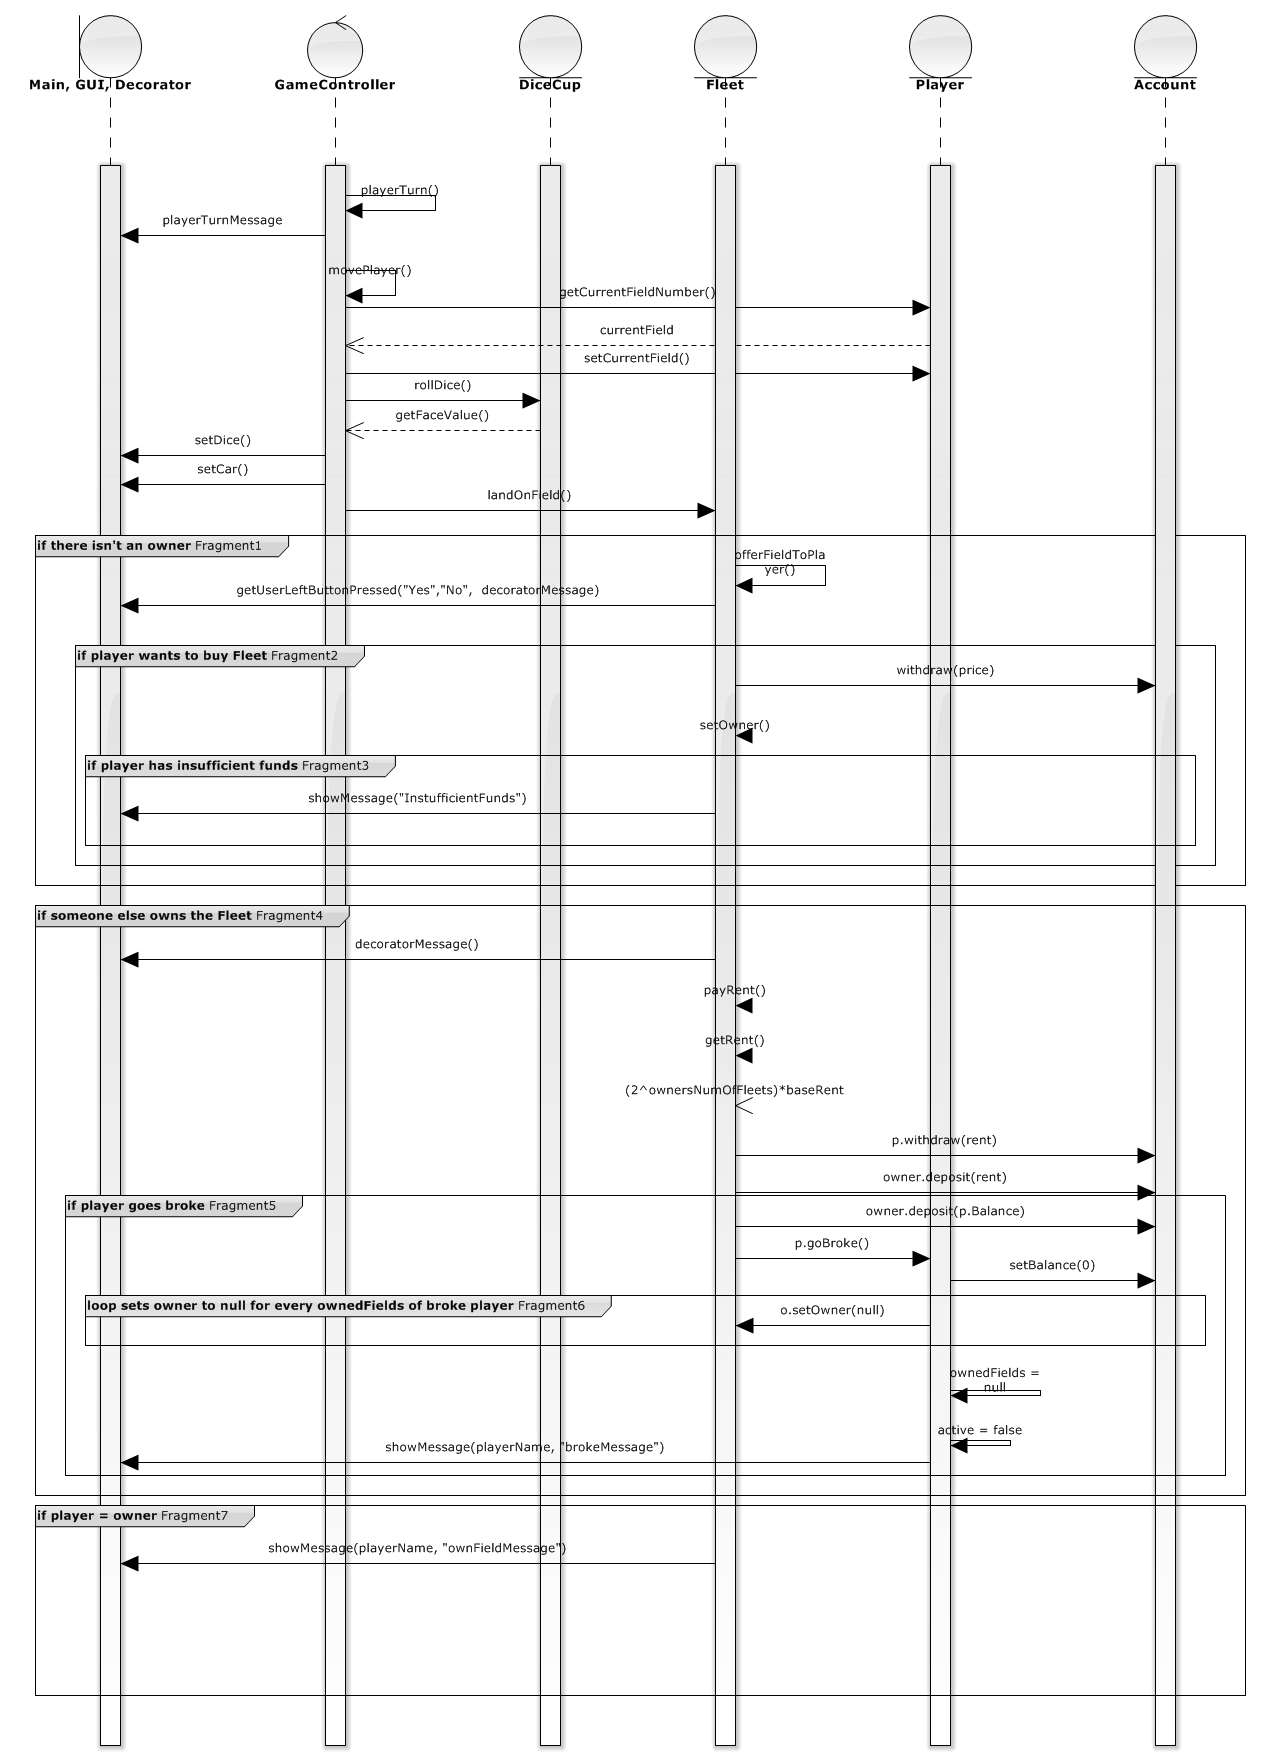
\includegraphics[width=\linewidth]{Sequencediagram3}
\caption{\emph{Sekvensdiagram 2}: Land on Field.}
\end{figure}
\FloatBarrier
Sekvensdiagrammerne er blevet lidt forsimplet for at fremme forståelse, og for
at ikke få for mange metodekald, der ikke ville bidrage til forståelsen af
diagrammet. Klasser der fungerer sammen og/eller ensartet er slået sammen.
Klasser af begrænset vigtighed for diagrammerne er også udeladt. Shuffler
indeholder en statisk metode, der blander felterne i starten af spillet. DiceCup
og Die arbejder så tæt sammen, at Die er undladt. Die er, som navnet hentyder,
en terning. Ownable er en superklasse til alle typer af felter, der kan ejes.
Fields er en superklasse til alle typer af felter. De forskellige typer af
felter, er slået sammen i det første diagram, og er kaldt Ownables, og i det
andet diagram, hvor vi viser landOnFleet, har vi valgt at udelukke de andre
felter, og ladt Fleet være den Ownable vi modellerer, da den er en subklasse af
“Ownable”. Mange returns er også blevet undladt for overskueligheden. Der er
brugt tre forskellige ikoner for klasser, nemlig Boundary, Control og Entity
(BCE), og man kan skelne dem ad ved at Boundary ser ud som, at den rører ved en
væg, Control har en lille pil på sig, og Entity ser ud som den rører ved noget
gulv. Derudover er der brugt to typer kasser. Loops, som repræsenterer loops,
hvis køringspremisser eller formål er beskrevet i den lille tekstboks øverst i
firkanten. Det andet er alt, som er kort for alternate. Dette viser et andet
udfald, der kan ske. Det bliver brugt til at vise ‘if’s og øverst i boksen er
præmissen for det givne if-alternativ anført.\\
\indent Det første sekvensdiagram viser et overordnet forløb af programmet, mens
det andet diagram viser alle de forskellige udfald, der kan opstå, når en spiller
lander på et  felt af typen Fleet. I det første er det på et lidt højere niveau
end i det  andet, da vi i det andet graver helt ind og ser på alle de
forskellige ting, der  kan ske, og ender derved med seks alternate-bokse.\\
\indent Hvis en spiller lander på en Fleet, er der allerede tre muligheder. Hvis
ingen ejer Fleet, skal det tilbydes til spilleren, hvorefter han kan vælge om han vil
købe den eller ej,  men der er en ekstra mulighed i det, at han måske ikke har
penge nok.\\
\indent Mulighed nummer to er, at en anden spiller ejer den. Så skal rent regnes
sammen, flyttes, og vi må se om spilleren er gået fallit. Hvis han er det, skal 
spilleren smides ud af spillet, og hans felter skal frigøres.\\
\indent Mulighed nummer tre er, at han selv ejer feltet, og så skal han bare
have en besked om, at han er landet på sit eget felt.
\section*{GRASP patterns}
\addcontentsline{toc}{subsection}{GRASP patterns}
Vi har forsøgt at arbejde med ‘responsibility driven design’ og implementeret
Controller, Creator, Information Expert, Low Coupling, High Cohesion og
Polymorphism.\\
\indent \emph{Controller} paradigmet er søgt overholdt ved vores GameController
klasse, der håndterer al spil logik og delegerer ansvaret videre. I vores projekt har vi
en lidt speciel statisk GUI, der tillader at vi tilgår den fra alle klasser i
programmet. Da den algoritme som felterne bruger er afhængig af spillerens
input fra GUI’en, har vi skullet vælge mellem at implementere 1) en løsning
hvor GameControlleren først tilgår feltet for at høre om det kan ejes, dernæst
om den kan købes eller er ejet, og dernæst eventuelt sætter ejeren for feltet,
eller 2) som vi i stedet har valgt - en løsning hvor felterne optræder som
subcontrollere og selv tilgår GUI’en for at håndtere hvad netop det felt gør.
På den måde bryder vi bevidst med BCE paradigmet (I det felterne også er
entities), men opnår en mere overskuelig løsning kodemæssigt og da relationen
er en ‘use’ relation med GUI’en øger det ikke coupling væsentligt. Cohesion
bevares også, da det er felterne selv, der logisk set kender reglerne for hvad
der sker når en spiller lander på feltet. Det er muligt at genskabe BCE, ved at
hvert felt får sin egen controller (hvilket ville være Pure Fabrication), men i
det givne tilfælde er det meget begrænset hvad en entity klasse skulle
indeholde, hvorfor vi har valgt at undlade at splitte klasserne op.\\
\indent \emph{Creator} er søgt overholdt ved at de klasser der ‘contains’ eller
‘aggregates’ andre klasser, også har ansvar for at instantiere dem. GameControlleren
instantierer DiceCup, der igen instantierer Die. Ligeledes oprettes Player med
account og Board med Fields. Vores Boundary klasse er et specialtilfælde, da den
er statisk, men initialiseres af GameControlleren, der har hovedansvaret for at
interagere med den.\\
\indent \emph{Information Expert} er søgt overholdt, ved kun at bevare
information og referencer i én klasse - den der er den mest oplagt til at indeholde
informationen. Vi har brudt med paradigmet enkelte steder for at opnå en mere
overskuelig løsning. Således har Gamecontrolleren en integer (playersLeft), der
holder styr på hvor mange players der er tilbage. Denne information er dubleret
fra players, der selv holder styr på om de er med i spillet med deres boolean
active. På samme måde ved både felterne hvem der ejer dem og playerne ved hvilke
felter de ejer. Dette giver desuden en højere coupling - da der er en reference
begge veje - Det giver også en lavere cohesion, da det nu er spredt over to
klasser. Man kan argumentere for at det stadig er logisk, da en grundejer kender
sine grunde og skødet på grunden ligeledes er påtrykt en ejer. Vi gør det under
alle omstændigheder for at opnå en simplere implementering af Fleet, der er nødt
til at vide hvor mange fleets ejeren har. Alternativet er at Fleet skal modtage
en reference til board og iterere over alle felterne for at afgøre hvor mange
fleets ejeren har. Et andet alternativ er at oprette en skødedatabase som kan
adspørges når behovet opstår - det ville svare til GRASP konceptet indirection
(og pure fabrication).\\
\indent \emph{Low Coupling} er opnået ved få koblinger pr. klasse - Dice er
koblet til DiceCup, Account til Player og Fields til Board, der igen er koblet
til GameController (se klasse diagram). GameControlleren har naturligt lidt
højere coupling - da  Dicecup, Players og Board (og Decorator) alle har
betydning for game-flowet. Det  er et acceptabelt antal bindinger - der
understøtter high cohesion. Vi  implementerer en undtagelse med et specifikt
felt - ‘Labor Camp’, der har en  reference til DiceCup. Det er gjort for at
kunne beregne lejen - uden at skulle  passe summen af øjne til feltet. En
alternativ løsning kunne være at  implementere DiceCup som en Singleton, der
kunne tilgås globalt. Som allerede  nævnt har vi en ‘use’ relation fra alle
felttyperne til GUI - idet de tilgår GUI  for at spørge spilleren om han vil
købe grunden eller betale et fast beløb eller  procent af formue i skat. Da det
er en ‘use’ relation er coupling stadig lav.\\
\indent \emph{High cohesion} er forsøgt bevaret ved at klassernes ansvarsområder
er nært beslægtede. Således har Die kun ansvar for terningernes øjne og at ‘slå’ et nyt
tilfældigt slag. Dicecup håndterer summen af øjnene og relaterede opgaver og så
fremdeles. Dette er i høj grad understøttet af low coupling, hvilket også
afspejles i at vi bryder med high cohesion samtidig med at vi bryder med low
coupling i tilfældet med ejerskabet af fields (som beskrevet ovenfor under
information expert)\\
\indent \emph{Polymorphism} er implementeret i vores felter. Her er
ensartede klassers kode forsøgt samlet i superklasser, således at vi genbruger
kode i højest muligt omfang og undgår at skrive den samme kode to gange. Det
afspejles tydeligst i decoratorMessage() metoden, der nedarver i 2 niveau og
sammensætter en ensartet besked til spilleren, sammensat af en besked om hvilket
felt man er landet på (bestemt af Field), en besked der afhænger af om feltet
kan ejes (bestemt af Ownable) og en besked fra selve feltet. Dette understøtter
reusability, idet ændringer i koden kun skal indføres et sted.

\newpage
\section{Implementering}
\section{Klasser}
\subsection{Main}
\subsection{Player}
\subsection{Account}
\subsection{Decorator}
\subsection{DiceCup}
\subsection{Die}
\subsection{GameController}
\subsection{Board}
\subsection{Field}
\subsection{Ownable}
\subsection{Tax}

\newpage
\section{Test}
\section*{BrugerTest}
\addcontentsline{toc}{subsection}{BrugerTest}
Vi har kørt nogle bruger tests, for at se om spillet opfører sig som forventet.
Vi har forsøgt at finde de fejl som gør at spillet af en eller anden grund giver
et forkert output, så som at spiller ikke går fallit når han skal, men får lov
at spille videre. Under \textbf{Bilag} kan man se screenshots fra en
brugertest.\\
\indent Under gennemførelsen af en brugertest, så det ud som at en vinder ikke
ikke blev præsenteret for spillerne. For at checke om controlleren kørte loopet
som finder vinderen, addede vi nogle linjer som blev printet hvis dele af loopen
blev kørt. Da vi så kørte den sidste brugertest fandt vi ud af at vinderen altid
spiller 1 selv om denne spiller var gået fallit
\textbf{\hyperref[bilag9]{Bilag9}}.
Fejlen var at da vi havde tilføjet den linje som blev printet, så havde vi glemt at omslutte if
statement med “\{“ således at alle spillere for den sags skyld kunne være
vindere. Ellers har vi kørt en fuldkommen brugertest hvor vi kommer igennem alle
scenarier vi kunne komme i tanker om. Bilag 1-9 er de scenarier vi forventer når
vi lander på et felt. Hvis man lander på et felt som ikke har en ejer, kan man
vælge at købe det, eller lade være \textbf{\hyperref[bilag1]{Bilag1}}.\\
\indent Hvis en spiller lander på et felt som er ejet af en anden, så får man
ikke mulighed for at købe det, men skal betale til ejeren
\textbf{\hyperref[bilag2]{Bilag2}}. Man kan også se at navnet på feltet og
navnet som bliver præsenteret som ejer af feltet er det samme. Det er den gule bil
(Christian) som er endt på Magnus felt og skal betale ham leje.\\
\indent Når man lander på det ene af tax felterne skal man have 2 muligheder for
at betale (enten 10\% eller 4000kr) \textbf{\hyperref[bilag7]{Bilag7}}. Mens det
andet tax felt kun skal kræve et bestemt beløb
\textbf{\hyperref[bilag3]{Bilag3}}. Disse felter får man ikke mulighed for at
købe, ligesom refugee heller ikke kan købes, men her får man penge
\textbf{\hyperref[bilag4]{Bilag4}}.\\
\indent Et andet scenarie er hvis du lander på dit eget felt, så skal der ikke
ske spilleren noget. Spilleren skal kun få at vide at han er landet på sit eget
felt \textbf{\hyperref[bilag5]{Bilag5}}, her kan nævnes at vi har gjort således
at felterne på GUI’en opdateres så man kan se hvem er ejer af feltet. Det er også
aktuelt når en spiller går fallit, så bliver den spiller fjernet som ejer af de
felter han havde og andre spillere får mulighed for at købe det
\textbf{\hyperref[bilag6]{Bilag6}}.\\
\indent Vi skulle også håndtere at en spiller ikke kan købe et felt for så at gå
fallit fordi han ikke har penge nok, og dette håndtere spillet
\textbf{\hyperref[bilag8]{Bilag8}}.
Spilleren får at vide at han ikke har penge nok, og spillet kører videre. dog
kan spilleren godt gå fallit når han lander på tax feltet hvor man vælge mellem
10\% og 4000 kr. Hvis han har råd til det ene, men ikke det andet, kan han
alligevel gå fallit ved forkert valg.\\
\indent To fejl som vi fandt ved brugertest, men som ikke er rettet, er hvis man 
skriver et grotesk langt navn for en spiller. Navnet bliver så langt at når det er
spillerens tur, dækker navnet “OK” knappen, og spillet kan ikke fortsættes
\textbf{\hyperref[bilag10]{Bilag10}}. Det skal altså være et virkelig, virkelig
langt navn. Hvis spillerne beslutter sig for at have samme navn, så bliver bliver to spillere
oprettet med hver sin konto, men på GUI’en har de samme farve bil
\textbf{\hyperref[bilag11]{Bilag11}}, altså er der kun en bil på brættet, men
som alligevel har to destinationer. Man kan derfor kun se bilen og balancen for den
ene spiller ad gangen.
\section*{Black Box (Junit)}
\addcontentsline{toc}{subsection}{Black Box (Junit)}
Vi har lavet en JUnit test class FieldJUnitTest, der tester LandOnField for alle
vores forskellige Field-klasser. Den opretter først sin egen test GUI, den skal
bruges da der er brugerinput i LandOnField, og derefter kører den en @test for
hver Field-type. Indlejret i disse test er også nogle test på ting fra Ownable,
såsom at gå fallit og lande på ens eget felt.\\
\indent Vi har kørt FieldJUnitTest løbene og brugt den til at rette adskillige
logiske fejl, til et punkt hvor FieldJUnitTest nu kører fejlfrit.
\section*{FURPS+}
\addcontentsline{toc}{subsection}{FURPS+}
FURPS+ er en forkortelse for Functionality, Usability, Reliability, Performance,
Supportability. FURPS+ er en god checkliste for at opnå et så godt program som
muligt, og ikke glemme nogle vigtige dele.
\begin{itemize}
  \item \textbf{functionality:} Vi har lavet et funktionelt spil, som opfylder
  alle kode mæssige krav, som for eksempel at bruge arv når vi programmerede felt
  klasserne og metoden landOnField i klassen Field.
  \item \textbf{Usability:} Spillet er brugervenligt, og der behøves ikke at
  læses nogen brugervejledning for at kunne gennemføre spillet. Dog skal man
  kende noget til matador regler for at forstå spillet, men du gennem spillet
  skal du kun trykke “OK” eller får du to valgmuligheder, hvor der er beskrevet
  hvad de betyder.
  \item \textbf{Reliability:} Gennem bruger tests og en stor J-Unit test, har vi
  elimineret alle de fejl, som opstår gennem de forventede scenarier. Som et af
  kravene har vi med J-Unit testet feltet af typen fleet for:
  \begin{itemize}
    \item at spiller ikke får fratrukket beløb når han lander på felt som han
    selv ejer.
    \item Når en spiller skal betale til en anden spiller, at den rigtige
    spiller får bestemt beløb og den anden fratrukket samme beløb.
    \item Når en spiller køber en fleet, bliver prisen af fleet fratrukket
    spillerens konto, og spiller bliver sat som ejer af feltet.
    \item Hvis en spiller er ejer af to fleets, så får den spiller som lander på
    en af hans fleet, fratrukket et beløb som svarer til $250 \cdot 2^(antal af
    fleets)$. Og ejeren tilføjet samme beløb.
    \item I tilfælde af at en spiller ikke har nok kapital ved landing på en
    andens spillers fleet, så bliver spillerens $balance = 0$, og
    $active = false$ (spilleren bliver inaktiv og er ikke mere del af
    spillet). Derefter bliver de penge som spilleren havde, overført til ejeren
    af fleet.
  \end{itemize}
  Så vi har et pålideligt spil, som ikke lukker ned uforventet.
  \item \textbf{Performance:} Dette har ikke været relevant faktor i vores spil.
  Spillet bruger så få ressourcer at vi har ikke haft brug for kørtids-analyser
  og optimering, spillet optager heller ikke mærkbar disk-space.
  \item \textbf{Supportability:} Vi har gjort en hel del ud af at fremtidssikre
  koden, så vi kan genbruge så meget som muligt af koden senere. For eksempel
  har vi undgået “hard coding”, og al tekst i spillet bliver gennem identifiers
  oversat, ved hjælp af decorator og properties filer, til meningsfyldt tekst.
  Properties filerne indeholder al tekst, og det gør det nemt at have overblik
  og ændre på teksten. Vi stødte dog på et problem, som vi løste med gøre
  felterne til subcontrollere, det gør koden lidt sværere at vedligeholde, da
  små ændringer i Decorator kan gøre at vi må gennemgå gamecontroller samt alle
  subcontrollerne for fejl.
  \item \textbf{+ (Plusset):} Spillet kræver at computeren har og kan køre en
  opdateret version af java og at mus og tastatur er tilkoblet. Spillet har
  ingen lyd, så det er ikke en nødvendighed. Ellers er der ikke nogen
  nævneværdige krav som spillet har til computeren.
\end{itemize}

\newpage
\section{Status og Konklusion}
Vi har alt i alt fremstillet et spil, der funktionelt set lever op til
specifikationerne - og tilføjer ekstra funktionalitet. Det kan spilles med
begrænsede forkundskaber, om end et kendskab til reglerne er nødvendigt for at
få det optimale udbytte. Det er pålideligt, men mangler et tjek for
brugernavnenes længde - så det er muligt at ødelægge brugeroplevelsen for sig
selv ved at indtaste grotesk lange brugernavne.\\
\indent Vi har taget nogle designbeslutninger, der skaber højere kobling og
bryder med BCE paradigmet. Det giver en overskuelig kode, men skaber det problem at det er
sværere at vedligeholde, idet ændringer i Decorator kan skabe behov for
ændringer i flere forskellige klasser.\\
\indent Idet formålet var at undgå for meget kode i vores GameController, kan
man forsøge at opnå det samme ved at indføre en dedikeret FieldController, der
delegeres ansvaret for sub use casen ‘Land on Field’. Vores dobbelte kobling
mellem Player og felterne, kan evt. løses ved at indføre et
‘tinglysningsregister’ - en (singleton) klasse, der kun har til opgave at holde
styr på ejerskabet af fields.


\newpage
\addcontentsline{toc}{section}{Referencer}
\bibliography{bibliografy}%% her indsættes referencerne

\newpage
\section{Bilag}
\begin{appendices}
\subsection*{Bilag 1 - }\label{Bilag1}
\addcontentsline{toc}{subsection}{Bilag 1 }

\subsection*{Bilag 2 - Samarbejdskontrakt}\label{Bilag2}
\addcontentsline{toc}{subsection}{Bilag 2 Samarbejdskontrakt}

\subsection*{Bilag 3 - Screendump af backlog under iteration 2}\label{Bilag3}
\addcontentsline{toc}{subsection}{Bilag 3 Backlog}

\subsection*{Bilag 4 - }\label{Bilag4}
\addcontentsline{toc}{subsection}{Bilag 4 PERT diagram}

\subsection*{Bilag 5 - }\label{Bilag5}
\addcontentsline{toc}{subsection}{Bilag 5}

\subsection*{Bilag 6 - }\label{Bilag6}
\addcontentsline{toc}{subsection}{Bilag 6}

\subsection*{Bilag 7 - }\label{Bilag7}
\addcontentsline{toc}{subsection}{Bilag 7}

\subsection*{Bilag 8 - }\label{Bilag8}
\addcontentsline{toc}{subsection}{Bilag 8}

\subsection*{Bilag 9 - }\label{Bilag9}
\addcontentsline{toc}{subsection}{Bilag 9}

\subsection*{Bilag 10 - }\label{Bilag10}
\addcontentsline{toc}{subsection}{Bilag 10}

\subsection*{Bilag 11 - }\label{Bilag11}
\addcontentsline{toc}{subsection}{Bilag 11}

\subsection*{Bilag 12 - }\label{Bilag12}
\addcontentsline{toc}{subsection}{Bilag 12}

\subsection*{Bilag 13 - }\label{Bilag13}
\addcontentsline{toc}{subsection}{Bilag 13}

\subsection*{Bilag 14 - }\label{Bilag14}
\addcontentsline{toc}{subsection}{Bilag 14}

\subsection*{Bilag 15 - }\label{Bilag15}
\addcontentsline{toc}{subsection}{Bilag 15}

\subsection*{Bilag 16 - }\label{Bilag16}
\addcontentsline{toc}{subsection}{Bilag 16}

\subsection*{Bilag 17 - }\label{Bilag17}
\addcontentsline{toc}{subsection}{Bilag 17}

\subsection*{Bilag 18 - }\label{Bilag18}
\addcontentsline{toc}{subsection}{Bilag 18}

\subsection*{Bilag 19 - }\label{Bilag19}
\addcontentsline{toc}{subsection}{Bilag 19}

\subsection*{Bilag 20 - }\label{Bilag20}
\addcontentsline{toc}{subsection}{Bilag 20}

\subsection*{Bilag 21 - }\label{Bilag21}
\addcontentsline{toc}{subsection}{Bilag 21}

\subsection*{Bilag 22 - }\label{Bilag22}
\addcontentsline{toc}{subsection}{Bilag 22}

\subsection*{Bilag 23 - }\label{Bilag23}
\addcontentsline{toc}{subsection}{Bilag 23}

\subsection*{Bilag 24 - }\label{Bilag24}
\addcontentsline{toc}{subsection}{Bilag 24}

\subsection*{Bilag 25 - }\label{Bilag25}
\addcontentsline{toc}{subsection}{Bilag 25}
\end{appendices}
\end{document}